\documentclass[10pt,twocolumn]{article}

\usepackage[T1]{fontenc}
\usepackage[utf8]{inputenc}
\usepackage{lmodern}
\usepackage{microtype}
\usepackage[margin=0.75in,columnsep=0.25in]{geometry}
\usepackage{amsmath,amssymb}
\usepackage{booktabs}
\usepackage{multirow}
\usepackage{xcolor}
\usepackage{graphicx}
\usepackage{tikz}
\usetikzlibrary{arrows.meta,positioning,calc}
\usepackage{pgfplots}
\pgfplotsset{compat=1.18}
\usepgfplotslibrary{groupplots}
\usepackage[numbers,sort&compress]{natbib}
\usepackage[hidelinks]{hyperref}
\usepackage{cleveref}
\usepackage{caption}
\captionsetup{font=small,labelfont=bf}

% One palette for every plot: baseline grey, OpenJet orange, NInfer blue.
\definecolor{cbase}{HTML}{7F7F7F}
\definecolor{cjet}{HTML}{E1812C}
\definecolor{cnin}{HTML}{3274A1}
\definecolor{cnin2}{HTML}{8CB5D6}
\definecolor{cgood}{HTML}{3A923A}

\title{\Large\bfseries Serving Qwen3.8-27B on a Single RTX~4090:\\
       2.5$\times$ Faster Decoding and Twice the Context at Baseline Precision}
\author{The qwen-4090-bench project\\\small\url{https://github.com/kineticsystem/qwen-4090-bench}}
\date{October 2026}

\newcommand{\PROFILETABLE}{\begin{table*}[t]
  \centering
  \caption{The retained server configurations, as started by the launcher scripts. Speeds in
           tok/s (speed-up over the baseline in parentheses); accuracy greedy, thinking off.}
  \label{tab:profiles}
  \resizebox{\textwidth}{!}{%
  \begin{tabular}{@{}llrccrrrrr@{}}
    \toprule
    Configuration & KV (K/V bits) & Context & Vision & Drafter & Short & Thinking & 29K prompt & GSM8K & HumanEval \\
    \midrule
    Baseline (llama.cpp) & q8\_0/turbo4 (8/4) & 128{,}000 & yes & MTP 2 & 89.6 & 84.2 & 76.0 & 97.2 & 96.3 \\
    OpenJet & q8 (8/8) & 131{,}072 & no & MTP 4 & 135.9 (1.52$\times$) & 130.2 & 110.7 & \OJGSM & \OJHE \\
    NInfer \texttt{precise} & rk8v4 (8/4) & 204{,}800 & yes & MTP 3 & 137.4 (1.53$\times$) & 129.7 & 122.2 & 97.6 & 95.1 \\
    NInfer \texttt{long} & E8 (4/4) & 262{,}144 & yes & MTP 3 & 139.0 (1.55$\times$) & 131.0 & 121.8 & 96.0 & 96.3 \\
    NInfer \texttt{fast} & E8 (4/4) & 192{,}512 & yes & DFlash2 7 & 166.0 (1.85$\times$) & 153.3 & 132.8 & 97.2 & 95.7 \\
    azllm & q8/q4 (8/4) & 241{,}664 & yes & DFlash2 7 & \textbf{228.6} (2.55$\times$) & \textbf{208.4} & \textbf{150.1} & 95.2 & 95.7 \\
    azllm, full window & q4/q4 (4/4) & 262{,}144 & yes & DFlash2 7 & \AZLS & \AZLT & \AZLL & \AZLG & \AZLH \\
    \bottomrule
  \end{tabular}}
\end{table*}
}
\newcommand{\OJGSM}{95.6}\newcommand{\OJHE}{96.3}
% azllm, full window (q4/q4, 262K): short, thinking, 29K, GSM8K, HumanEval
\newcommand{\AZLS}{228.8 (2.55$\times$)}\newcommand{\AZLT}{195.1}\newcommand{\AZLL}{145.6}\newcommand{\AZLG}{96.8}\newcommand{\AZLH}{95.7}
\begin{document}
\maketitle

\begin{abstract}
We study how fast, and with how much context, a dense 27B-parameter hybrid model can be served
to a single user on one 24\,GB RTX~4090 without losing precision. Starting from a tuned
llama.cpp setup (89.6\,tok/s, 128K context), we compare three specialized engines on
Qwen3.8-27B: OpenJet, a persistent megakernel that reads the same GGUF file; NInfer, a dedicated
engine with its own 4/5-bit weights; and azllm, a tqLLM fork that reads rotated 4.3-bit weights.
Both NInfer and azllm draft with DFlash2, a block-diffusion model. azllm decodes at
228.6\,tok/s on short prompts (2.55$\times$), up to 3.1$\times$ on code, and 2.47$\times$ in
thinking mode; NInfer reaches 1.85$\times$ and OpenJet 1.52$\times$. On the same 98K positions
of code, azllm's weights lose 0.46\% in log-likelihood against the baseline's and NInfer's
1.78\%, and GSM8K and HumanEval stay within the noise of greedy decoding. A capacity map over KV
formats, drafters and the vision tower, verified by filling each context with real source code,
shows that the model's full 262{,}144-token window fits with vision in two engines. A 4-bit KV
cache costs 0.16\% (azllm) to 0.82\% (NInfer) in log-likelihood on code, an effect invisible to
exact recall of code at 252K tokens. We release launcher scripts for every configuration.
\end{abstract}

\section{Introduction}
\label{sec:intro}

A dense 27-billion-parameter model quantized to about 4.5 bits per weight occupies roughly
17\,GB, which leaves about 6\,GB of a 24\,GB consumer GPU for the key--value (KV) cache, the
activations and the engine's own buffers. At batch size one, decoding is bound by memory
bandwidth: every generated token reads every weight once. On an RTX~4090 (1008\,GB/s), this
puts plain autoregressive decoding of such a model at about 50--60 tokens per second, whatever
the engine.

Two levers move this limit without changing the weights. \emph{Speculative decoding}
 lets a cheap drafter propose several tokens that the target model
verifies in one forward pass, which costs about as much memory traffic as a single token. And
\emph{engine specialization} removes the overheads a general engine carries: kernel launches,
host round trips and generic memory layouts. A third lever, \emph{KV-cache quantization}, does
not make short prompts faster, but decides how much context fits in the memory that is left.

This report studies the three levers on one concrete case: Qwen3.8-27B, a hybrid
Gated-DeltaNet/attention model with a built-in multi-token-prediction (MTP) head, served for a
single user who mostly writes code, on one RTX~4090. We start from a tuned llama.cpp setup and
ask three questions:

\begin{enumerate}
  \item How much faster can single-stream decoding get, at unchanged accuracy?
  \item How much context fits on the card, with and without the vision encoder, without the
        server failing?
  \item What does a 4-bit KV cache cost in precision on code, compared with the 8-bit keys
        and 4-bit values of the starting setup?
\end{enumerate}

We compare four engines: llama.cpp with the TurboQuant KV types \citep{llamacpp,turboquant}
(the baseline), the OpenJet persistent megakernel \citep{openjet}, the RTX~4090 port of NInfer
\citep{ninfer,ninfer4090} with both MTP and the DFlash2 block-diffusion drafter,
 and azllm \citep{azllm}, a fork of tqLLM \citep{tqllm} that reads
rotated TurboQuant weights. All measurements come from one machine, in throw-away containers,
with scripts that are part of this work.

\paragraph{Contributions.}
\begin{itemize}
  \item A like-for-like measurement of decode speed, accuracy and context capacity for four
        engines serving the same model on the same GPU, including thinking mode and a 29K-token
        prompt.
  \item A comparison of three 4-bit weight files on exactly the same code positions, showing
        that a rotated 4.3-bit format predicts code within 0.5\% of a 5.2-bit k-quant file.
  \item A capacity map: the largest context each configuration (engine, KV type, drafter,
        vision on or off) accepts, each verified by filling the context with real code and
        querying it.
  \item A measurement of the cost of KV-cache quantization on code perplexity at 64K and 128K
        context, and on exact recall of code at up to 252K tokens.
  \item Ready-to-run server scripts for every configuration; the recommended one serves
        2.5$\times$ faster than the baseline with 1.9$\times$ its context and vision, and the
        full 262K window with a 4-bit KV cache.
\end{itemize}

\section{Background}
\label{sec:background}

\paragraph{The model.}
Qwen3.8-27B interleaves Gated DeltaNet layers, whose state is a fixed-size
matrix per head, with full-attention layers, whose KV cache grows with the context. Only the
attention layers pay per-token memory, which is why a 27B model can hold a 256K-token context in
a few gigabytes. The recurrent state, however, cannot simply be truncated when a draft token is
rejected: engines must either snapshot it or replay the accepted tokens.

\paragraph{Speculative decoding.}
A drafter proposes $k$ tokens; the target model scores all of them in one pass and keeps the
longest prefix that matches its own choice (greedy) or passes a rejection test (sampling), so
the output distribution is unchanged. The speed-up depends on the
mean number of tokens accepted per pass and on how cheap the drafter and the $(k{+}1)$-token
verification are. Qwen3.8-27B ships an MTP head that drafts one token per
step from the target's last hidden state. DFlash2 is a separate small
block-diffusion model that drafts a whole block in one pass, conditioned on the target's hidden
states, and is accepted further on predictable text such as code.

\paragraph{KV-cache quantization.}
The KV cache can be stored in fewer bits than the activations that produce it.
 Keys are more sensitive than values, since an error in a key changes
every attention weight it takes part in. Rotations spread outliers across channels before
quantization, and lattice codes such as $E_8$
quantize eight values jointly at a lower error than scalar rounding at the same rate.
Table~\ref{tab:kvtypes} lists the formats compared in this work.

\begin{table}[t]
  \centering
  \caption{KV-cache formats compared. Bits are per element, scales excluded.}
  \label{tab:kvtypes}
  \resizebox{\columnwidth}{!}{%
  \begin{tabular}{@{}llccl@{}}
    \toprule
    Engine & Format & K bits & V bits & Encoding \\
    \midrule
    llama.cpp & \texttt{q8\_0}/\texttt{q8\_0} & 8 & 8 & blocks of 32, one scale \\
    llama.cpp & \texttt{q8\_0}/\texttt{turbo4} & 8 & 4 & TurboQuant values (baseline) \\
    OpenJet & \texttt{q8} & 8 & 8 & as \texttt{q8\_0} \\
    NInfer & \texttt{int8} & 8 & 8 & groups of 64 \\
    NInfer & \texttt{rk8v4} & 8 & 4 & rotated keys, groups of 64 \\
    NInfer & \texttt{rk4v4-e8} & 4 & 4 & rotated, $E_8$ lattice keys \\
    \bottomrule
  \end{tabular}}
\end{table}

\section{Systems Under Test}
\label{sec:systems}

Figure~\ref{fig:systems} shows the four engines side by side. All four serve an
OpenAI-compatible HTTP API, run one request at a time, and verify drafts exactly.

\begin{figure*}[t]
  \centering
  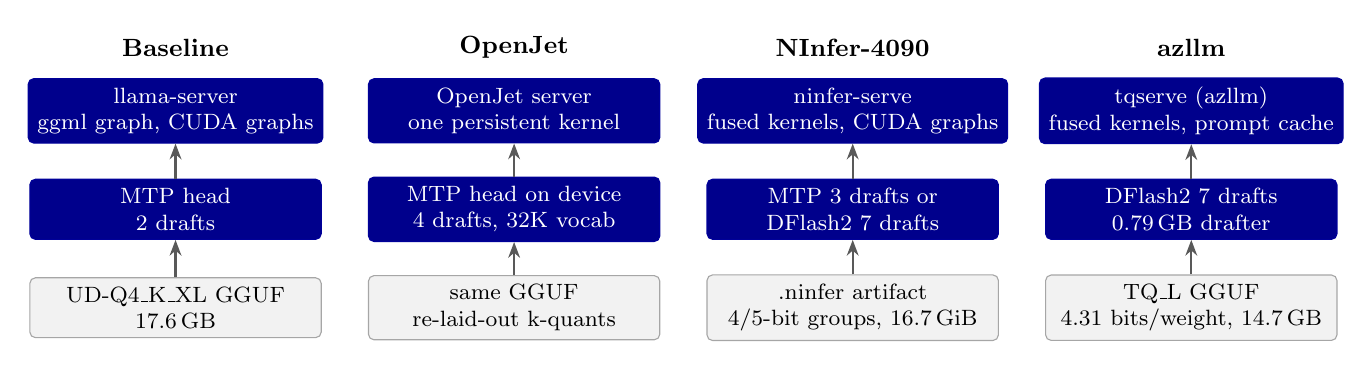
\begin{tikzpicture}[
      font=\footnotesize,
      box/.style={draw=blue!60!black, fill=blue!55!black, text=white, rounded corners=2pt,
                  minimum width=3.7cm, minimum height=0.75cm, align=center},
      weights/.style={draw=gray!70, fill=gray!10, rounded corners=2pt,
                      minimum width=3.7cm, minimum height=0.75cm, align=center},
      arr/.style={-{Stealth[length=2mm]}, gray!70!black, thick}]
    % columns
    \node[box] (l1) at (0,0) {llama-server\\ggml graph, CUDA graphs};
    \node[box] (l2) at (0,-1.25) {MTP head\\2 drafts};
    \node[weights] (l3) at (0,-2.5) {UD-Q4\_K\_XL GGUF\\17.6\,GB};
    \node[box] (o1) at (4.3,0) {OpenJet server\\one persistent kernel};
    \node[box] (o2) at (4.3,-1.25) {MTP head on device\\4 drafts, 32K vocab};
    \node[weights] (o3) at (4.3,-2.5) {same GGUF\\re-laid-out k-quants};
    \node[box] (n1) at (8.6,0) {ninfer-serve\\fused kernels, CUDA graphs};
    \node[box] (n2) at (8.6,-1.25) {MTP 3 drafts or\\DFlash2 7 drafts};
    \node[weights] (n3) at (8.6,-2.5) {.ninfer artifact\\4/5-bit groups, 16.7\,GiB};
    \node[box] (a1) at (12.9,0) {tqserve (azllm)\\fused kernels, prompt cache};
    \node[box] (a2) at (12.9,-1.25) {DFlash2 7 drafts\\0.79\,GB drafter};
    \node[weights] (a3) at (12.9,-2.5) {TQ\_L GGUF\\4.31 bits/weight, 14.7\,GB};
    \foreach \c in {l,o,n,a} { \draw[arr] (\c3) -- (\c2); \draw[arr] (\c2) -- (\c1); }
    \node[font=\small\bfseries] at (0,0.8) {Baseline};
    \node[font=\small\bfseries] at (4.3,0.8) {OpenJet};
    \node[font=\small\bfseries] at (8.6,0.8) {NInfer-4090};
    \node[font=\small\bfseries] at (12.9,0.8) {azllm};
  \end{tikzpicture}

  \caption{The four engines. Grey: the weights each one reads; blue: the drafter and the
           serving layer. OpenJet reads the baseline's own GGUF file; NInfer and azllm need their
           own weight files, both of which come with a DFlash2 drafter.}
  \label{fig:systems}
\end{figure*}

\paragraph{Baseline: llama.cpp with TurboQuant.}
The starting point is the TurboQuant fork of llama.cpp \citep{turboquant}, built from commit
\texttt{a3d5603d1} for \texttt{sm\_89}, serving Unsloth's \texttt{UD-Q4\_K\_XL} GGUF
 with flash attention, MTP speculation with two drafts, keys in
\texttt{q8\_0}, values in \texttt{turbo4} and a 128{,}000-token context. The vision projector
stays in host memory.

\paragraph{OpenJet Engine.}
OpenJet \citep{openjet} runs a whole speculative cycle (verification of $1+k$ tokens, lm-head,
acceptance, MTP catch-up and the next $k$ drafts) inside one cooperative kernel separated by
software grid barriers. It reads the same GGUF, keeps the k-quant encodings, and rolls the
DeltaNet state back by replaying accepted drafts from a small ring instead of snapshotting it.
The draft lm-head is restricted to the 32{,}768 most frequent tokens; verification uses the full
vocabulary. It is text only, and its KV cache is \texttt{f16} or \texttt{q8}.

\paragraph{NInfer-4090.}
NInfer \citep{ninfer} is a C++20/CUDA engine written for the Qwen3.6/3.8 family; we use the
\texttt{sm\_89} port \citep{ninfer4090}. It loads its own groupwise artifact
(4- and 5-bit weight groups, 8-bit output head) and offers MTP or DFlash2 drafting, a paged KV
cache in several formats (Table~\ref{tab:kvtypes}), prefix reuse at message boundaries, and an
optional vision tower. Its image targets CUDA~13.1; on the 580 driver (CUDA~13.0) it runs through
minor-version compatibility once the container's requirement check is disabled.

\paragraph{azllm (tqLLM).}
tqLLM \citep{tqllm} is a C++/CUDA engine for Qwen models stored in its own rotated
TurboQuant weight types, a GGUF extension that stock llama.cpp cannot load. azllm \citep{azllm}
is a fork that changes only the serving layer (streaming with tools, live timings, prompt-cache
bookmarks); we found it through a practitioner's report. We serve the
\texttt{TQ\_L} weights (4.31 bits per weight, 14.7\,GB, against about 5.2 for the other two
files) with a DFlash2 drafter quantized to TQ3 (0.79\,GB) and a 65{,}536-token
draft vocabulary. KV formats pair rotated 8- or 4-bit keys with 8-, 4-, 3- or 2-bit values; the
prompt cache keeps the previous request's KV so that a repeated prefix is not read again. The
vision projector must be F16 or F32. \texttt{TQ\_L} embeds Qwen's official chat template, which
fails on tool calls whose arguments arrive as a JSON string, so our launcher passes the fixed
template that the \texttt{TQ3\_4S-v2} file embeds.

\paragraph{Engines not retained.}
A Windows-oriented fork of NInfer-4090 has the same single-token decode rate
(about 52\,tok/s) and its KV modes are already merged into the port we use. vLLM and SGLang with
4-bit AWQ/GPTQ weights leave too little memory for a useful KV cache on 24\,GB, and NVFP4 needs
Blackwell. Lucebox runs DFlash2 inside a llama.cpp-based server but publishes
no RTX~4090 figure, and the one community report of DFlash2 in llama.cpp on this card we found
gives 73--75\,tok/s.

\section{Method}
\label{sec:method}

\paragraph{Hardware and isolation.}
One NVIDIA GeForce RTX~4090 (24\,GB, 450\,W stock limit, PCIe~3.0~x16), an Intel Core
i9-10900K and 62\,GB of RAM, under Ubuntu with driver 580.178. Every engine is built and run in a
throw-away Docker container; the model files are mounted read-only. One server runs at a time.

\paragraph{Decode speed.}
A client streams each answer and computes decode speed as $(n-1)/(t_\text{last}-t_\text{first})$,
where $n$ is the number of generated tokens and $t$ the arrival times of the first and last
streamed tokens, so prompt processing is excluded and every engine is measured the same way. The
short benchmark has six prompts (two coding tasks, a short story, a technical explanation, a word
problem and a table), up to 1024 tokens each, with the sampling the model card recommends
(temperature 0.6, top-$p$ 0.95, top-$k$ 20, min-$p$ 0, presence penalty 0) and a fixed seed. We
report the mean over the prompts. Final configurations were repeated three times; with a fixed
seed the repetitions agree within 1\,tok/s, while separate server starts vary by about 5\%.
The long-prompt benchmark prefixes three questions with 29{,}005 tokens of CUDA source code.

\paragraph{Accuracy.}
GSM8K (first 250 test problems) and HumanEval
(all 164, pass@1, run against the official tests), greedy, thinking off.

\paragraph{Context capacity.}
For NInfer, the memory planner decides at startup whether a configuration fits, so we
binary-search the largest \texttt{--max-context} (in steps of 4096 tokens) that starts. For
OpenJet, which allocates at startup and fails with \texttt{cudaMalloc} out of memory, we do the
same. A start is not proof: each retained configuration is then filled to within 2--3\% of its
limit with real source code and queried (next paragraph); we call a context \emph{usable} only
if the server answers every question and is still alive afterwards.

\paragraph{KV precision.}
Two measurements. (i) Code perplexity: NInfer's offline evaluator scores 359{,}927 tokens of
CUDA/C++ source with windows of 64K (stride 32K) or 128K (stride 64K) tokens, for each KV format;
we patched its command line to accept the rotated and lattice formats that the server already
supports. For llama.cpp, \texttt{llama-perplexity} scores the same text in 64K chunks. For
azllm, \texttt{tqkld} first dumps the top-16 log-probabilities of the \texttt{q8} cache as a
reference, then scores the other formats against it (KL divergence, top-1 agreement and NLL),
on four 64K chunks of which the last 32K positions are scored. Within each engine, the most
precise format it offers is the reference. (ii) Long-context recall: the prompt holds up to 252K tokens of
llama.cpp source, then twelve questions ask the model to copy, exactly, the first 16 lines of
the body of a named function in a named file, at depths spread from 10\% to 98\%. A function
qualifies only if its name is defined once in its file. We report the share of lines copied
exactly.

\paragraph{Weight precision.}
The three weight files are compared on the same 98{,}304 positions: chunks 1--3 of 64K tokens,
last 32K of each, with 8-bit keys and values. \texttt{llama-perplexity} with 64K chunks,
\texttt{tqkld --tail 32768}, and NInfer's windows starting at 64K, 128K and 192K (stride 32K)
all score exactly these positions, and the three tokenizers produce the same 359{,}928 tokens. The
comparison includes each engine's own arithmetic, not the weights alone, and there is no BF16
reference: it tells which pipeline predicts the code best, not which is closest to the original
model.

\section{Results}
\label{sec:results}

\subsection{Decode speed at short context}

Figure~\ref{fig:speed} ranks the configurations on the six short prompts. Raising the
baseline's MTP drafts from two to five gains 19\%; beyond five, rejected drafts cost more than
they bring. OpenJet, with four MTP drafts on the baseline's own GGUF, reaches 134.7\,tok/s
(1.50$\times$). NInfer with MTP is slightly faster (137--140\,tok/s) and with seven DFlash2
drafts reaches 166.9\,tok/s (1.86$\times$). azllm, with seven DFlash2 drafts on its smaller
\texttt{TQ\_L} weights, reaches 228.6\,tok/s: 2.55$\times$ the baseline and 1.37$\times$
NInfer.

\begin{figure}[t]
  \centering
  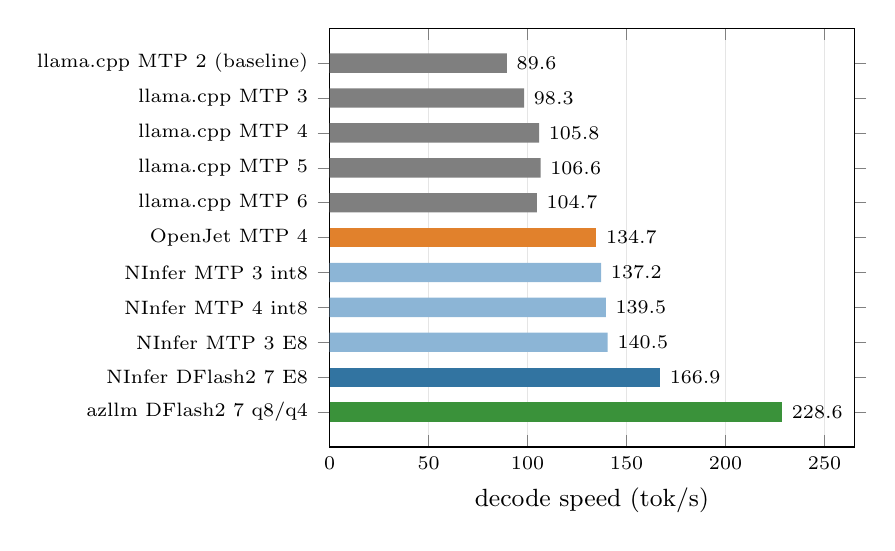
\begin{tikzpicture}
    \begin{axis}[
        xbar, width=0.68\columnwidth, height=6.9cm, bar width=7pt,
        xmin=0, xmax=265, xlabel={decode speed (tok/s)},
        symbolic y coords={b2,b3,b4,b5,b6,oj,nm3,nm4,nm3e,nd7,az},
        ytick={b2,b3,b4,b5,b6,oj,nm3,nm4,nm3e,nd7,az}, y dir=reverse,
        yticklabels={llama.cpp MTP 2 (baseline), llama.cpp MTP 3, llama.cpp MTP 4,
                     llama.cpp MTP 5, llama.cpp MTP 6, OpenJet MTP 4, NInfer MTP 3 int8,
                     NInfer MTP 4 int8, NInfer MTP 3 E8, NInfer DFlash2 7 E8, azllm DFlash2 7 q8/q4},
        yticklabel style={font=\scriptsize}, xticklabel style={font=\scriptsize},
        xlabel style={font=\small},
        nodes near coords, nodes near coords style={font=\scriptsize},
        every axis plot/.append style={draw=none, bar shift=0pt},
        xmajorgrids, grid style={gray!20}]
      \addplot[fill=cbase] coordinates {(89.6,b2) (98.3,b3) (105.8,b4) (106.6,b5) (104.7,b6)};
      \addplot[fill=cjet] coordinates {(134.7,oj)};
      \addplot[fill=cnin2] coordinates {(137.2,nm3) (139.5,nm4) (140.5,nm3e)};
      \addplot[fill=cnin] coordinates {(166.9,nd7)};
      \addplot[fill=cgood] coordinates {(228.6,az)};
    \end{axis}
  \end{tikzpicture}

  \caption{Mean decode speed over six short prompts, recommended sampling, thinking off.
           Grey: llama.cpp; orange: OpenJet; blue: NInfer; green: azllm.}
  \label{fig:speed}
\end{figure}

The gain depends on the text (Figure~\ref{fig:perprompt}). On the two coding prompts and the
word problem, azllm runs 2.9--3.1$\times$ faster than the baseline and NInfer 2.1--2.3$\times$;
on free prose, which no drafter predicts well, the gains fall to 1.70$\times$ and
1.28$\times$. Thinking mode (effort \emph{medium}) gives 208.4 against 84.2\,tok/s for azllm
(2.47$\times$) and 153.3 for NInfer (1.82$\times$).

\begin{figure}[t]
  \centering
  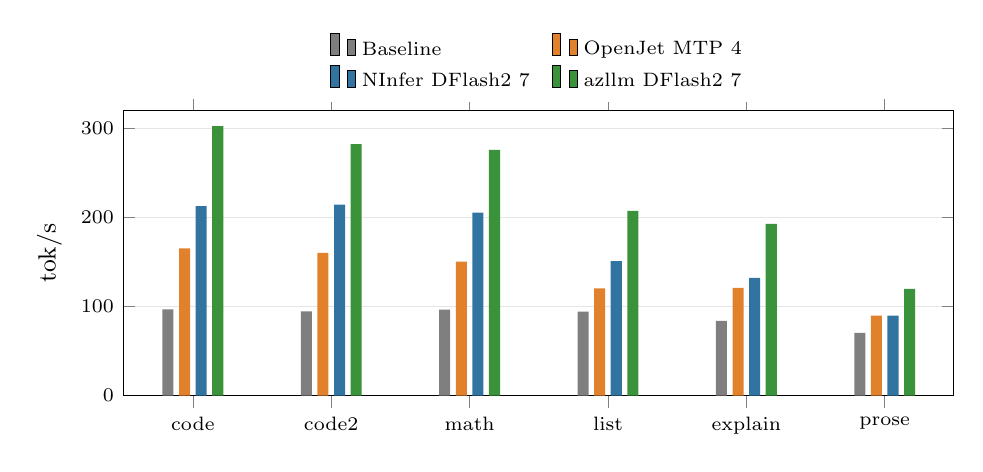
\begin{tikzpicture}
    \begin{axis}[
        ybar, width=\columnwidth, height=5.2cm, bar width=4pt,
        ymin=0, ymax=320, ylabel={tok/s}, ylabel style={font=\small},
        symbolic x coords={code,code2,math,list,explain,prose},
        xtick=data, xticklabel style={font=\scriptsize}, yticklabel style={font=\scriptsize},
        legend style={font=\scriptsize, at={(0.5,1.03)}, anchor=south, draw=none, legend columns=2, /tikz/every even column/.append style={column sep=6pt}},
        legend cell align=left, enlarge x limits=0.1,
        every axis plot/.append style={draw=none}, ymajorgrids, grid style={gray!20}]
      \addplot[fill=cbase] coordinates {(code,97.0) (code2,94.7) (math,96.6) (list,94.6) (explain,84.0) (prose,70.5)};
      \addplot[fill=cjet] coordinates {(code,165.4) (code2,160.5) (math,150.7) (list,120.6) (explain,121.1) (prose,90.1)};
      \addplot[fill=cnin] coordinates {(code,212.9) (code2,214.7) (math,205.7) (list,151.2) (explain,132.3) (prose,90.1)};
      \addplot[fill=cgood] coordinates {(code,302.7) (code2,282.6) (math,276.1) (list,207.7) (explain,193.1) (prose,120.0)};
      \legend{Baseline, OpenJet MTP 4, NInfer DFlash2 7, azllm DFlash2 7}
    \end{axis}
  \end{tikzpicture}

  \caption{Decode speed per prompt. Structured output (code, a worked problem, a table) gains
           most; a short story gains least.}
  \label{fig:perprompt}
\end{figure}

\paragraph{Number of drafts.}
Figure~\ref{fig:drafts} sweeps the number of draft tokens. NInfer's DFlash2 peaks at five to
seven drafts and drops sharply beyond; azllm's DFlash2 rises up to seven and stays flat up to
ten. MTP, which drafts one token per step, peaks at three to five. On NInfer the KV format makes
no measurable difference at short context (DFlash2 7: 166.9\,tok/s with E8, 166.7 with int8);
on azllm neither (228.5 with \texttt{q8/q4}, 230.7 with \texttt{q4/q4}).

\begin{figure}[t]
  \centering
  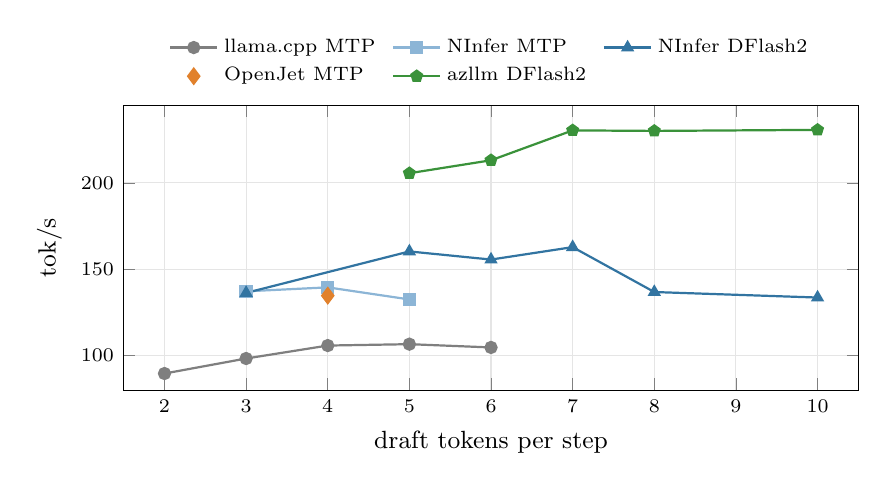
\begin{tikzpicture}
    \begin{axis}[
        width=0.9\columnwidth, height=5.2cm, xmin=1.5, xmax=10.5, ymin=80, ymax=245,
        xlabel={draft tokens per step}, ylabel={tok/s},
        xlabel style={font=\small}, ylabel style={font=\small},
        ticklabel style={font=\scriptsize}, xtick={2,3,...,10},
        legend style={font=\scriptsize, at={(0.5,1.03)}, anchor=south, draw=none, legend columns=3, /tikz/every even column/.append style={column sep=4pt}},
        legend cell align=left, grid=major, grid style={gray!20}]
      \addplot[cbase, thick, mark=*] coordinates {(2,89.6) (3,98.3) (4,105.8) (5,106.6) (6,104.7)};
      \addplot[cnin2, thick, mark=square*] coordinates {(3,137.2) (4,139.5) (5,132.5)};
      \addplot[cnin, thick, mark=triangle*] coordinates {(3,136.3) (5,160.3) (6,155.6) (7,162.8) (8,136.8) (10,133.6)};
      \addplot[cjet, only marks, mark=diamond*, mark size=3pt] coordinates {(4,134.7)};
      \addplot[cgood, thick, mark=pentagon*] coordinates {(5,205.6) (6,213.1) (7,230.4) (8,230.1) (10,230.7)};
      \legend{llama.cpp MTP, NInfer MTP, NInfer DFlash2, OpenJet MTP, azllm DFlash2}
    \end{axis}
  \end{tikzpicture}

  \caption{Decode speed against the number of draft tokens. NInfer DFlash2 points use E8 KV,
           except 3 and 10 drafts (int8 KV at 96K); azllm points use \texttt{q8/q4} KV at 128K
           without vision.}
  \label{fig:drafts}
\end{figure}

\subsection{Accuracy}

Table~\ref{tab:profiles} lists accuracy next to speed for the retained configurations. With
greedy decoding and thinking off, all engines solve 238--244 of the 250 GSM8K problems and
156--158 of the 164 HumanEval problems. OpenJet, which reads exactly the baseline's weights,
solves four GSM8K problems fewer than the baseline, and azllm solves more with its 4-bit cache
(242) than with its 8-bit one (238), so differences of this size are the noise of greedy decoding
on near-ties. To compare the weights themselves we turn to perplexity.

\PROFILETABLE

\subsection{Weight precision}

Figure~\ref{fig:weights} compares the three weight files on the same 98{,}304 positions of code.
Taking the baseline's UD-Q4\_K\_XL as the reference (0.4330 nats per token), azllm's
\texttt{TQ\_L} loses 0.46\% and NInfer's groupwise artifact 1.78\%. The ranking holds in every
chunk. \texttt{TQ\_L} is the smallest file (4.31 against about 5.2 bits per weight), so its
rotated format buys both speed and precision. Prefilling with FP16 instead of int8 activations
changes azllm's result by 0.0002 nats, so the gap comes from the weights, not the prefill path.

\begin{figure}[t]
  \centering
  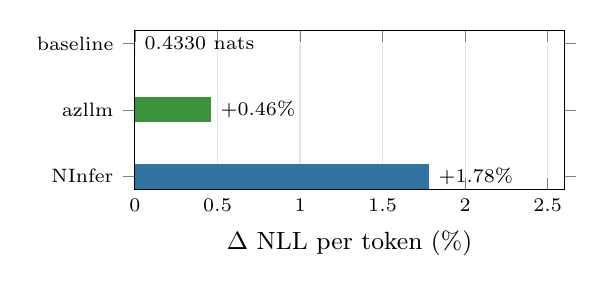
\begin{tikzpicture}
  \begin{axis}[
      xbar, width=0.58\columnwidth, height=3.6cm, bar width=9pt,
      xmin=0, xmax=2.6, xlabel={$\Delta$ NLL per token (\%)},
      xlabel style={font=\small},
      symbolic y coords={ud,tq,ni}, ytick={ud,tq,ni}, y dir=reverse,
      yticklabels={baseline, azllm, NInfer},
      yticklabel style={font=\scriptsize}, xticklabel style={font=\scriptsize},
      point meta=explicit symbolic, nodes near coords, nodes near coords style={font=\scriptsize, anchor=west},
      every axis plot/.append style={draw=none, bar shift=0pt}, xmajorgrids, grid style={gray!20}]
    \addplot[fill=cbase] coordinates {(0,ud) [0.4330 nats]};
    \addplot[fill=cgood] coordinates {(0.46,tq) [+0.46\%]};
    \addplot[fill=cnin] coordinates {(1.78,ni) [+1.78\%]};
  \end{axis}
\end{tikzpicture}

  \caption{Mean NLL per token on 98{,}304 positions of C++/CUDA code (32K--64K tokens of
           context each), relative to the baseline's weights; 8-bit KV in every engine. Lower is
           better.}
  \label{fig:weights}
\end{figure}

\subsection{Context capacity}

Figure~\ref{fig:capacity} maps the largest context each configuration accepts. Three factors
decide it: the KV format (int8 to rk8v4 to E8 roughly doubles NInfer's capacity), the drafter
(NInfer's DFlash2 keeps its own KV cache and costs 57--111K tokens), and the vision tower
(16--33K tokens). OpenJet allocates a fixed 2048-token prefill scratch; shrinking it to 512
tokens raises its ceiling from 131{,}072 to 147{,}456 tokens with \texttt{q8} keys and values,
and it has no 4-bit KV and no vision. azllm reaches the full native window, with vision, with
\texttt{q4/q4} KV, and 241{,}664 tokens with \texttt{q8/q4}. Near its limits it moves the token
embeddings and a copy of the LM head to host memory; decode speed is unchanged (228.5\,tok/s at
241{,}664 tokens with vision, 230.4 at 131{,}072 without).
These limits leave each engine's default free memory, 768\,MiB for azllm. With 2\,GB left free
for a desktop on the same card, azllm starts with at most 151{,}552 tokens with \texttt{q8/q4} KV
and 233{,}472 with \texttt{q4/q4}: near the \texttt{q8/q4} limit, what no longer fits is the
full-size prefill buffers, not the KV cache.

\begin{figure*}[t]
  \centering
  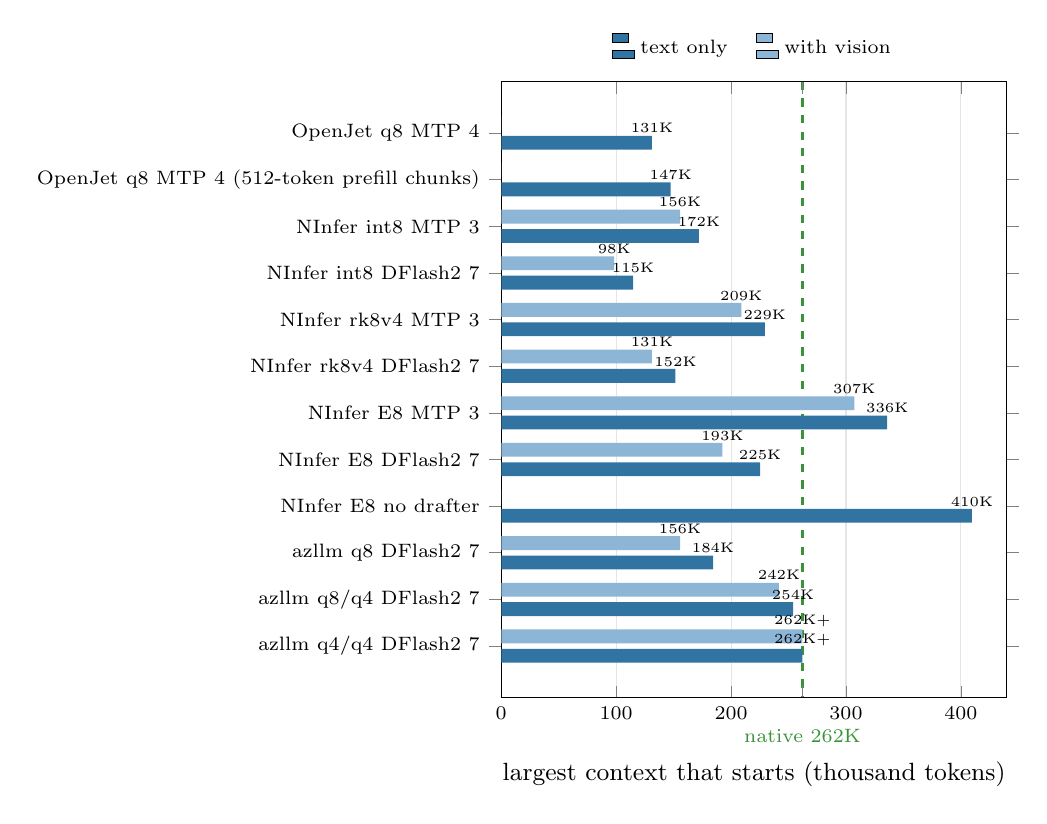
\begin{tikzpicture}
  \begin{axis}[
      xbar, width=0.66\textwidth, height=9.4cm, bar width=5pt,
      xmin=0, xmax=440, xlabel={largest context that starts (thousand tokens)},
      xlabel style={font=\small},
      symbolic y coords={oj,ojc,ni8m,ni8d,nr8m,nr8d,ne8m,ne8d,ne8n,a8,a84,a44},
      ytick=data, y dir=reverse,
      yticklabels={OpenJet q8 MTP 4, OpenJet q8 MTP 4 (512-token prefill chunks),
                   NInfer int8 MTP 3, NInfer int8 DFlash2 7, NInfer rk8v4 MTP 3,
                   NInfer rk8v4 DFlash2 7, NInfer E8 MTP 3, NInfer E8 DFlash2 7,
                   NInfer E8 no drafter, azllm q8 DFlash2 7, azllm q8/q4 DFlash2 7, azllm q4/q4 DFlash2 7},
      yticklabel style={font=\scriptsize}, xticklabel style={font=\scriptsize},
      legend style={font=\scriptsize, at={(0.5,1.02)}, anchor=south, draw=none,
                    legend columns=2, /tikz/every even column/.append style={column sep=8pt}},
      legend cell align=left,
      point meta=explicit symbolic,
      nodes near coords, nodes near coords style={font=\tiny},
      every axis plot/.append style={draw=none}, xmajorgrids, grid style={gray!20},
      extra x ticks={262.144}, extra x tick labels={native 262K},
      extra x tick style={grid=major, major grid style={cgood, thick, dashed},
                          tick label style={text=cgood, font=\scriptsize, yshift=-8pt}}]
    \addplot[fill=cnin] coordinates {(131.1,oj) [131K] (147.5,ojc) [147K] (172.0,ni8m) [172K]
        (114.7,ni8d) [115K] (229.4,nr8m) [229K] (151.6,nr8d) [152K] (335.9,ne8m) [336K]
        (225.3,ne8d) [225K] (409.6,ne8n) [410K]
        (184.3,a8) [184K] (254.0,a84) [254K] (262.1,a44) [262K+]};
    \addplot[fill=cnin2] coordinates {(0,oj) [] (0,ojc) [] (155.6,ni8m) [156K] (98.3,ni8d) [98K]
        (208.9,nr8m) [209K] (131.1,nr8d) [131K] (307.2,ne8m) [307K] (192.5,ne8d) [193K] (0,ne8n) []
        (155.6,a8) [156K] (241.7,a84) [242K] (262.1,a44) [262K+]};
    \legend{text only, with vision}
  \end{axis}
\end{tikzpicture}

  \caption{Largest context accepted at startup, binary-searched in steps of 4096 tokens. The
           baseline's own setting is 128{,}000 tokens. OpenJet has no vision; the no-drafter E8
           row is shown text only; azllm's search stopped at the native window. The dashed line
           marks the model's native window; going past it would need RoPE scaling, which we did
           not test.}
  \label{fig:capacity}
\end{figure*}

\paragraph{Does the context really fit?}
A configuration that starts may still fail later, when a long prompt allocates prefill buffers.
Table~\ref{tab:fill} fills each retained configuration to near its limit and queries it. Every
server answered every question and stayed up, and the vision-enabled ones still described an
image afterwards. The baseline slows to 55\,tok/s at 121K tokens; NInfer stays above
106\,tok/s at 252K, and azllm answers at 162\,tok/s with 252K tokens in context. azllm's prompt
cache also shows here: after reading 219K tokens in 147\,s, the next request, the same prompt
plus 15K tokens, was read in 15\,s.

\begin{table}[t]
  \centering
  \caption{Full-context runs: prompt filled with source code, twelve questions asking for the
           first 16 lines of a named function. ``Exact'': answers with all 16 lines in place;
           ``Similar'': mean line-sequence similarity; decode speed while answering.}
  \label{tab:fill}
  \small
  \setlength{\tabcolsep}{3pt}
  \begin{tabular}{@{}lrrrr@{}}
    \toprule
    Configuration & Prompt & Exact & Similar & tok/s \\
    \midrule
    Baseline, vision & 121{,}375 & 11/12$^a$ & 0.989 & 55.3 \\
    OpenJet q8, 147K & 142{,}807 & 12/12 & 1.000 & 125.1 \\
    NInfer fast, vision & 184{,}886 & 12/12 & 1.000 & 114.7 \\
    NInfer precise, vision & 196{,}772 & 12/12 & 1.000 & 109.9 \\
    NInfer precise, text & 221{,}095 & 11/12$^b$ & 0.995 & 106.3 \\
    NInfer long, vision & 252{,}392 & 12/12 & 1.000 & 108.4 \\
    azllm \texttt{q8/q4}, vision & 233{,}777 & 11/12$^a$ & 0.989 & 132.1 \\
    azllm \texttt{q4/q4}, vision & 252{,}392 & 12/12 & 1.000 & 161.8 \\
    \bottomrule
  \end{tabular}\\[2pt]
  \parbox{\columnwidth}{\scriptsize $^a$ The function contains the literal text
  \texttt{<|im\_start|>}, which llama.cpp and azllm read as a special token and drop from the
  output; the rest was exact. $^b$ The answer omitted the first line, \texttt{try \{}, and copied
  the other 15 exactly.}
\end{table}

\subsection{What a 4-bit KV cache costs on code}

The recall test of Table~\ref{tab:fill} does not separate the KV formats: at 98K tokens, int8,
rk8v4 and E8 all copy every requested line exactly, and the 4-bit formats of both NInfer and
azllm still do at 252K. Perplexity is more sensitive (Figure~\ref{fig:kvppl}). In NInfer, int8
is indistinguishable from bf16, rk8v4 costs 0.13\% (0.15\% at 128K context), and E8 with 4-bit
keys 0.82\% (0.79\%). In llama.cpp, the baseline's \texttt{turbo4} values cost 0.11\%. In
azllm, \texttt{q8/q4} costs 0.04\% and \texttt{q4/q4} 0.16\%, with a mean KL divergence from the
\texttt{q8} cache of 0.0008 and 0.0019 nats and top-1 agreement of 99.5\% and 99.1\%. azllm's
4-bit keys, rotated and quantized in blocks of 32 with one FP16 scale, are five times cheaper
than NInfer's $E_8$-lattice keys.

\begin{figure}[t]
  \centering
  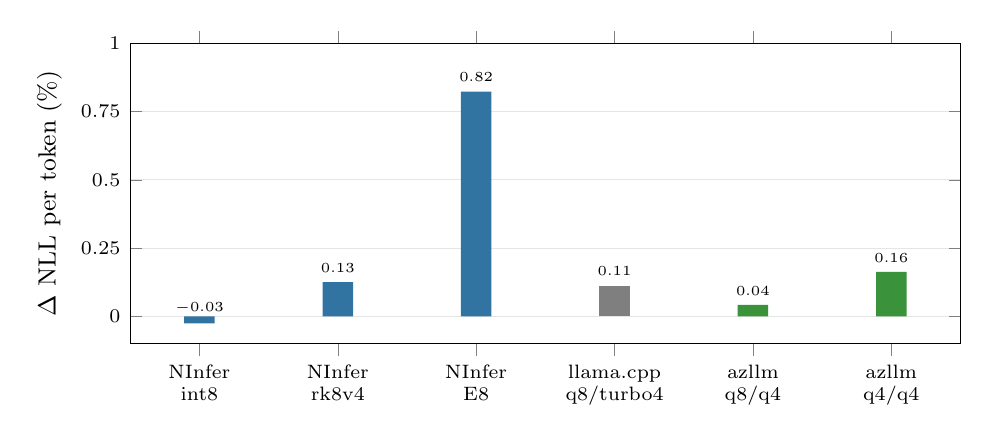
\begin{tikzpicture}
  \begin{axis}[
      ybar, width=\columnwidth, height=5.4cm, bar width=11pt,
      ymin=-0.1, ymax=1.0, ytick={0,0.25,0.5,0.75,1},
      ylabel={$\Delta$ NLL per token (\%)}, ylabel style={font=\small},
      symbolic x coords={ni8,nr8,ne8,lt4,a84,a44},
      xtick={ni8,nr8,ne8,lt4,a84,a44}, xticklabels={NInfer\\int8, NInfer\\rk8v4, NInfer\\E8, llama.cpp\\q8/turbo4, azllm\\q8/q4, azllm\\q4/q4},
      xticklabel style={font=\scriptsize, align=center},
      yticklabel style={font=\scriptsize},
      enlarge x limits=0.1, clip=false,
      point meta=explicit symbolic, nodes near coords, nodes near coords style={font=\tiny},
      every axis plot/.append style={draw=none, bar shift=0pt}, ymajorgrids, grid style={gray!20}]
    \addplot[fill=cnin] coordinates {(ni8,-0.025) [$-$0.03] (nr8,0.126) [0.13] (ne8,0.823) [0.82]};
    \addplot[fill=cbase] coordinates {(lt4,0.113) [0.11]};
    \addplot[fill=cgood] coordinates {(a84,0.042) [0.04] (a44,0.163) [0.16]};
  \end{axis}
\end{tikzpicture}

  \caption{Cost of each KV format on code: relative change of the mean NLL per token against
           the most precise format of the same engine (NInfer: bf16; llama.cpp: q8\_0/q8\_0;
           azllm: q8), 64K windows with the last 32K positions scored. Lower is better.}
  \label{fig:kvppl}
\end{figure}

\section{Discussion}
\label{sec:discussion}

\paragraph{Where the speed comes from.}
Single-token decode of a 17\,GB model is bound by memory bandwidth at about 50\,tok/s on this
card, and every engine sits close to that bound without speculation (NInfer 50.5\,tok/s,
llama.cpp 45.9, as reported by the NInfer port). All of the gain therefore comes from three
places: how many tokens a verification pass accepts (the drafter), how cheap the drafter and the
$(k{+}1)$-token verification are (the engine), and how many bytes a pass reads (the weights).
DFlash2 accepts longer runs than the model's own MTP head on structured text, and both
specialized engines make verification cheap. azllm adds the third lever: its weight file is
16\% smaller than the baseline's, and on code it predicts nearly as well, which is unusual for a
smaller file and points to the value of rotation before quantization.

\paragraph{Context is a memory budget.}
On 24\,GB, the weights take 15--18\,GB and everything else competes for the rest: the KV cache,
the drafter and its own cache, the vision tower, prefill buffers and CUDA graphs. Two choices
dominate. 4-bit keys double the context, and a block-diffusion drafter with its own KV cache
costs up to 111K tokens in NInfer. azllm's drafter is small (0.79\,GB), so its fastest
configuration also reaches the full window. Startup checks are not enough: we filled every
retained configuration with real code before calling its context usable.

\paragraph{Precision of a 4-bit KV cache.}
For code, the KV cache matters at long range, where an error in a key shifts attention to the
wrong line. Exact recall of 16-line functions did not separate any format, even at 252K tokens.
Perplexity did: a 4-bit cache costs between 0.16\% (azllm) and 0.82\% (NInfer's $E_8$), against
0.11\% for the baseline's 4-bit values. The difference between the two 4-bit formats is larger
than the difference between 4- and 8-bit keys within azllm, so the format matters more than the
bit count.

\paragraph{Limitations.}
\begin{itemize}
  \item One machine, one GPU, one session. Accuracy runs are single greedy passes; the GSM8K and
        HumanEval differences we report are of the size of their noise.
  \item There is no BF16 reference model: the weight comparison ranks three 4-bit pipelines,
        each with its own arithmetic, not their distance to the original model.
  \item We did not evaluate long agentic sessions with tools. Field reports describe looping
        with four or more MTP drafts in NInfer during long tool-calling runs;
 our NInfer profiles use three, and azllm limits repetition by
        default (\texttt{--repeat-limit 256}). A tool-call smoke test passed on azllm with the
        fixed template.
  \item Speeds were measured with the card at its stock 450\,W limit. The host reset once,
        without a GPU error in the log, during back-to-back compute-bound runs; thereafter a
        guard logged temperatures every 10\,s (peak 80\,$^\circ$C) and never had to pause.
  \item The capacity limits leave each engine's default free memory on the GPU (768\,MiB for
        azllm), but our card also drives the display, whose desktop holds about 1\,GB and grows
        as windows open. Next to it, azllm with \texttt{q8/q4} KV refuses 221{,}184 tokens. Our
        packaged servers keep 2\,GB free and serve 151{,}552 tokens (\texttt{q8/q4}) and
        233{,}472 (\texttt{q4/q4}); the KV cache is reserved whole at start, so the room is for
        the desktop and the CUDA graphs. NInfer and OpenJet lose more, down to 77{,}824 and
        65{,}536 tokens; their limits were measured from the free memory, which the desktop
        moves by up to 400\,MiB between starts.
  \item azllm and NInfer are young projects maintained by few people, and both need weight
        files of their own.
\end{itemize}

\section{Conclusion}
\label{sec:conclusion}

On one RTX~4090, Qwen3.8-27B can be served 2.5$\times$ faster than a tuned llama.cpp setup,
with almost twice its context and vision, at the same precision on code. The engine that
achieves it, azllm, combines a DFlash2 block-diffusion drafter, a specialized CUDA engine and a
rotated 4.3-bit weight format that predicts code within 0.5\% of the baseline's 5.2-bit file.
Its 4-bit KV cache costs 0.16\% in log-likelihood and fits the full 262K-token window with the
vision tower. We release launcher scripts for every configuration measured here, served
behind llama-swap \citep{llamaswap}, which starts the engine a request asks for.


\bibliographystyle{plainnat}
\bibliography{refs}

\onecolumn
\appendix
\section{Reproducing the Measurements}
\label{app:repro}

All paths are relative to \texttt{\textasciitilde/repo/qwen-research}. Each engine runs in a
throw-away container; one server at a time.

\begin{table}[h]
  \centering
  \small
  \begin{tabular}{@{}lp{0.74\textwidth}@{}}
    \toprule
    What & Command \\
    \midrule
    Start a server (port 8084) & \texttt{./qwen-baseline.sh start}, \texttt{./qwen-openjet.sh start}, \\
                               & \texttt{./qwen-ninfer.sh start long|fast|precise}, \texttt{./qwen-azllm.sh start [--kv q4/q4 --ctx 262144]} \\
    Short-prompt speed & \texttt{bench/bench.py --url http://127.0.0.1:8084 --model Qwen3.8-27B --label X [--think] [--greedy]} \\
    29K-token prompt & \texttt{bench/bench.py... --long 100000} \\
    GSM8K and HumanEval & \texttt{bench/evalacc.py --url... --label X} \\
    Full-context recall & \texttt{bench/longctx.py --url... --tokens N --n-questions 12 --lines 16} \\
    NInfer capacity & \texttt{bench/probe-ninfer.sh "label|--kv-dtype rk4v4-e8 --spec mtp --draft-tokens 3"} \\
    OpenJet capacity & \texttt{DOCKER\_ENV="-e MK\_PF\_CAP=512" bench/probe-openjet.sh "label|--kv q8 -d 4"} \\
    Code perplexity, NInfer & \texttt{bench/ppl-ninfer.sh 65536 32768 int8 rk8v4 rk4v4-e8} \\
    Code perplexity, llama.cpp & \texttt{bench/ppl-llama.sh 65536 q8\_0/q8\_0 q8\_0/turbo4} \\
    azllm capacity & \texttt{bench/probe-tqllm.sh "label|--kv q8/q4"}, then \texttt{bench/check-tqllm-fit.sh} \\
    KV cost, azllm & \texttt{bench/kld-tqllm.sh q8 q8/q4 q4/q4} \\
    Weight comparison & \texttt{bench/weights-compare.sh}, then \texttt{python3 bench/weights-compare.py} \\
    Temperature guard & \texttt{nohup bench/thermal-guard.sh \&} \\
    \bottomrule
  \end{tabular}
\end{table}

\noindent For NInfer, \texttt{bench/bench.py}, \texttt{evalacc.py} and \texttt{longctx.py} take
\texttt{--no-think top}: NInfer rejects \texttt{chat\_template\_kwargs} and reads
\texttt{enable\_thinking} and \texttt{reasoning\_effort} as top-level request fields.
Raw results are in \texttt{results/}: \texttt{bench\_summary.jsonl} (speed),
\texttt{accuracy.jsonl}, \texttt{longctx.jsonl} (with every answer),
\texttt{ninfer-capacity.txt}, \texttt{openjet-capacity.txt}, \texttt{tqllm-capacity.txt},
\texttt{tqllm-fit.txt}, \texttt{ppl-ninfer.txt}, \texttt{ppl-llama.txt}, \texttt{tqkld.txt},
\texttt{weights-compare-table.txt} and \texttt{thermal.log}.

\paragraph{A note on stability.} The host reset once without any GPU error in the kernel log,
during back-to-back compute-bound perplexity runs at the card's stock 450\,W limit. The scripts
now pause 60\,s between heavy runs and a guard pauses the containers above 83\,$^\circ$C on the
GPU or 90\,$^\circ$C on the CPU; no further reset occurred and the guard never triggered.

\end{document}
